\chapter{System Design and Implementation}

\section{Global System Design}

\section{Model View Controller}
As mentioned earlier, we are using the Play Framework. 
This frameworks follows the Model View Controller (MVC) architectural pattern applied to the Web architecture\cite{playframework_mvc}.
This pattern splits the application into separate layers: the Presentation layer and the Model layer. 
The Presentation layer is further split into a View and a Controller layer.

\subsection{Controller}
The \textbf{Controller} responds to events (typically user actions) and processes them, and may also invoke changes on the model.
In a Web application, events are typically HTTP requests: a Controller listens for HTTP requests, extracts relevant data from the 'event', such as query string parameters, request headers... 
And applies changes on the underlying model objects.
\\\\
In Play, a Controller is a Java class where each public, static, method is an \textbf{action}.
An action is a Java entry point invoked when a HTTP Request is received.
The Java code from the Controller class is not really object oriented: it is mainly procedural code.
The action method extracts relevant data from the HTTP request, reads or updates the model objects, and sends back a result which is wrapped into an HTTP Response.

\subsection{Model}
The \textbf{Model} is the domain-specific representation of the information on which the application operates.
Domain logic adds 'meaning' to raw data (e.g., calculating if today is the user's birthday, or the totals, taxes, and shipping charges for a shopping cart).
 Most applications use a persistent storage mechanism such as a database to store data.
MVC does not specifically mention the data access layer because it is understood to be underneath, or encapsulated by, the Model.
\\\\
In Play, the domain model object layer is a set a Java classes using all the object oriented features available from the Java language. 
It contains data structures and operations on which the application operates. 
Whenever model objects need to be saved into a persistent storage, they may contain some glue artefacts like JPA annotations or SQL statements.

\subsection{View}
The \textbf{View} renders the model into a form suitable for interactions, typically a user interface.
Multiple views can exist for a single model, for different purposes.
In a Web application the view is usually rendered in a 'Web format' like HTML, XML or JSON.
However there are some cases where the view can be expressed in a binary form, e.g. dynamically rendered chart diagrams.
\\\\
In Play, most of the application views are generated using an efficient templating system provided by play. 
The Controller gets some interesting data from the model layer, and then applies a template to decorate these objects. 
This packages contains HTML, XML, JSON and other template files with special directives used to dynamically generate the model representation.
\\
\begin{figure}[h]
  \centering
    \captionsetup{justification=centering}
    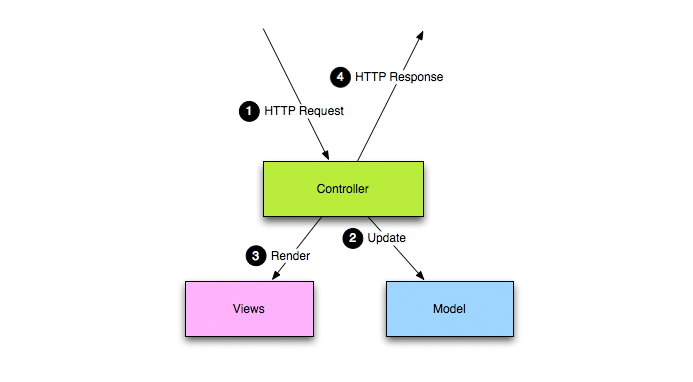
\includegraphics[width=\textwidth]{play_mvc}
    \caption{Play Framework MVC structure}
  \label{play_mvc_image}
\end{figure}